\documentclass{standalone}
\usepackage{tikz}
\begin{document}
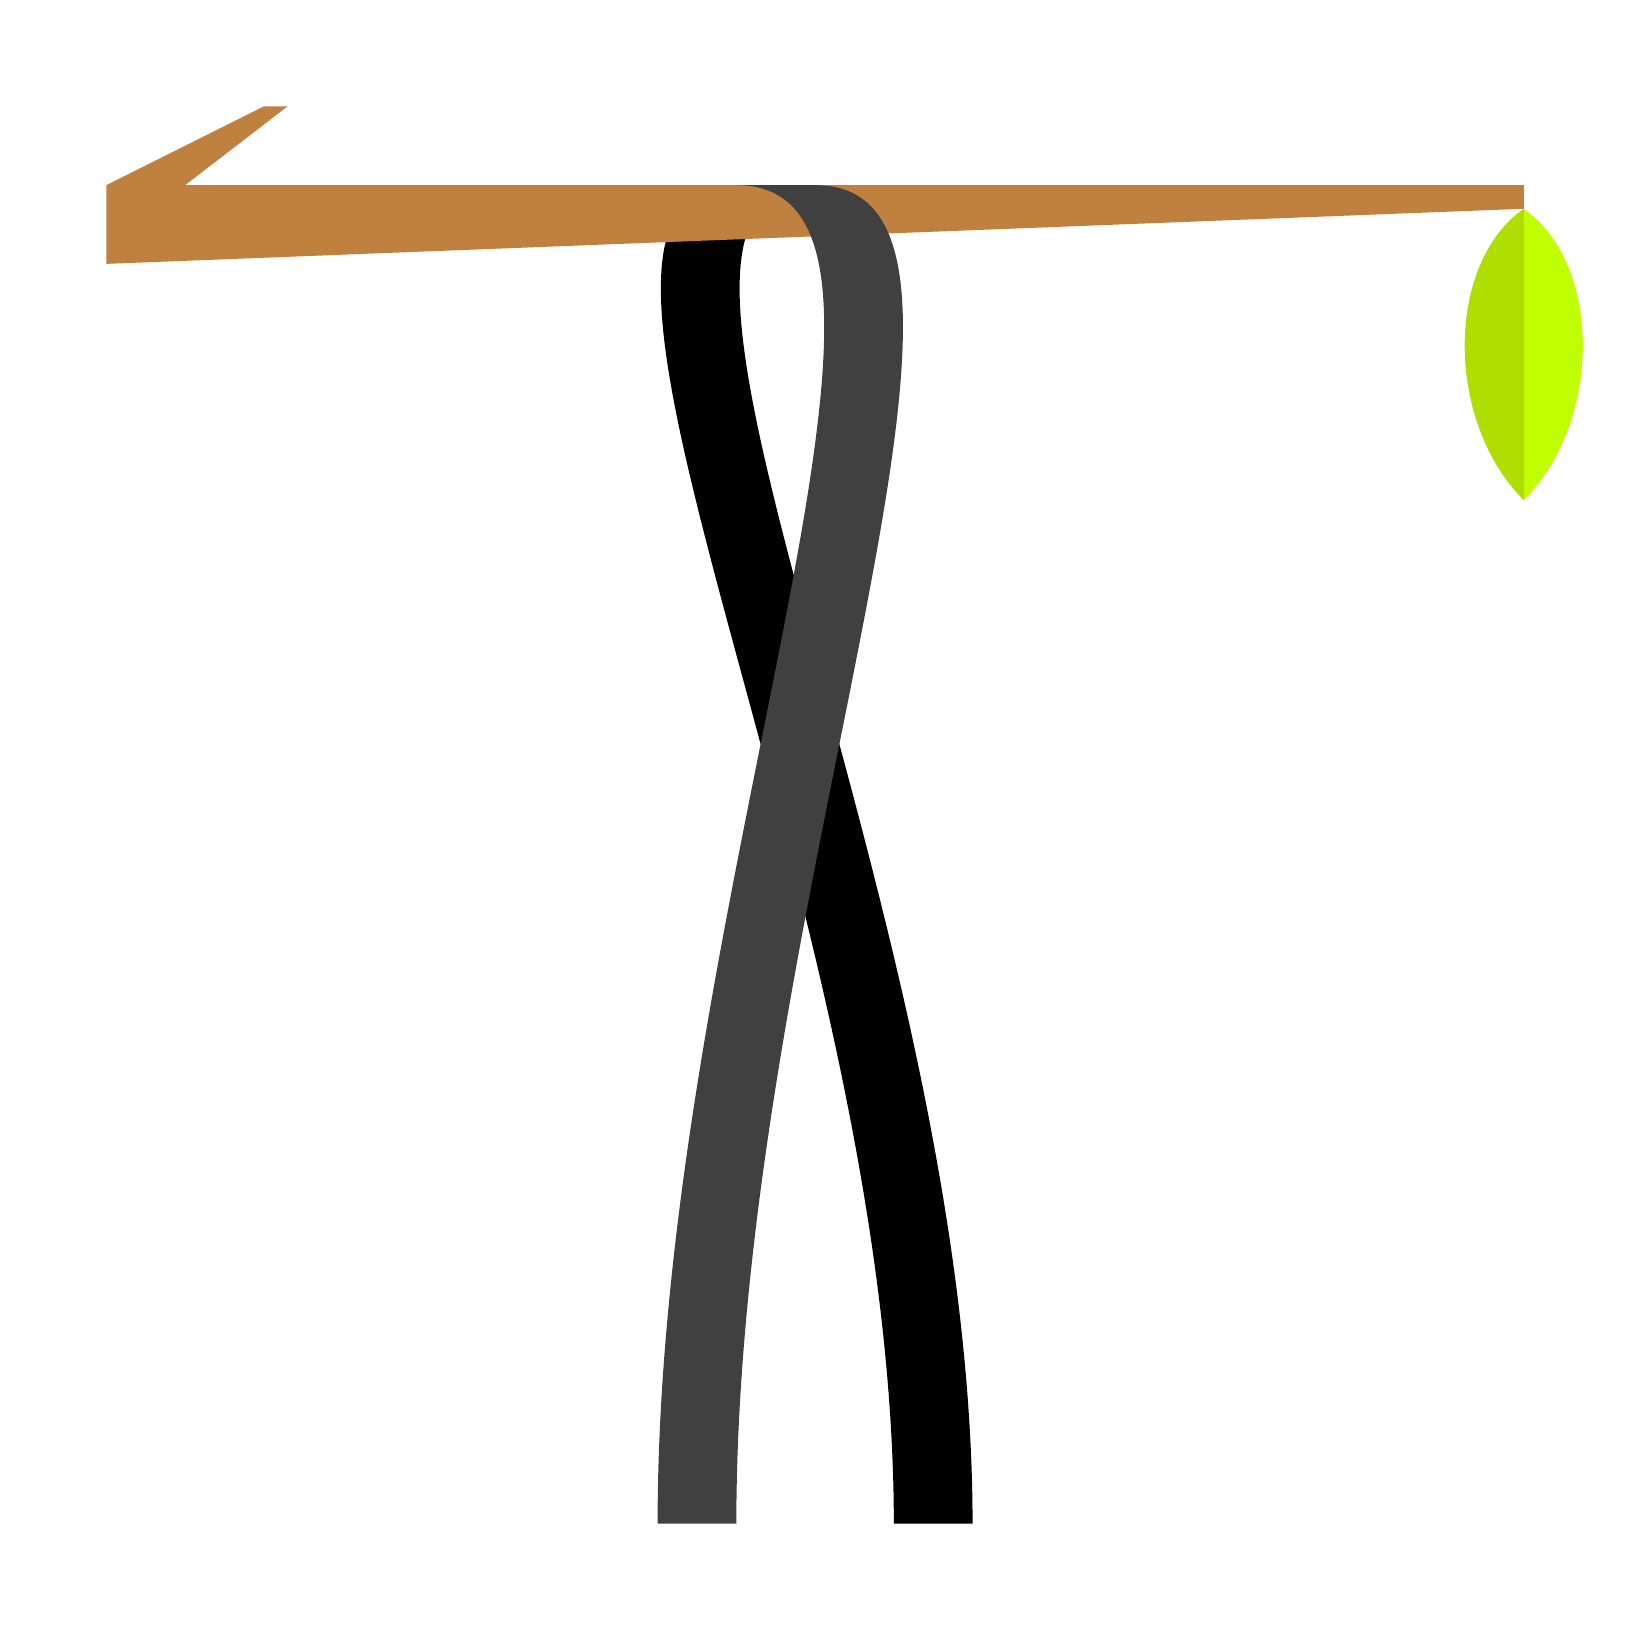
\begin{tikzpicture}
    \useasboundingbox (0,0) rectangle (20,20);
    \fill[black] (12,1) to[controls={(12,9) and (7,18)}] (10,18)--(9,18) to[controls={(6,18) and (11,9)}] (11,1)--cycle;
    \fill[brown] (1,17)--(19,17.7)--(19,18)--(2,18)--(3.3,19)--(3,19)--(1,18)--cycle;
    \fill[darkgray] (9,1) to[controls={(9,9) and (13,18)}] (10,18)--(9,18) to[controls={(12,18) and (8,9)}] (8,1)--cycle;
    \fill[lime] (19,14) to[controls={(20,15) and (20,17)}] (19,17.7)--cycle;
    \fill[lime!75!olive] (19,17.7) to[controls={(18,17) and (18,15)}] (19,14)--cycle;
\end{tikzpicture}
\end{document}
